{\fontsize{12pt}{22pt} \textbf{Projectors}\par}

\vspace{5mm}

Definition: a projector $p$ is a linear application such that: \\

(i) There exists a decomposition of the initial set in two supplementary sets: \\
$$E = F \oplus G$$
$$p: E \to F$$
$$x = x_F + x_G \to x_F$$

$G$ is the "projection direction"
Also, $F = Im(p)$ and $G = Ker(p)$ \\

(ii) $p$ is \textit{idempotent}:
$$p \circ p=p$$
Intuitively, it means that applying $p$ a second time doesn't change anything. \\

Definition (bis) : a square matrix $P$ is called a projection matrix if it is equal to its square, i.e. if $P^2 = P$.


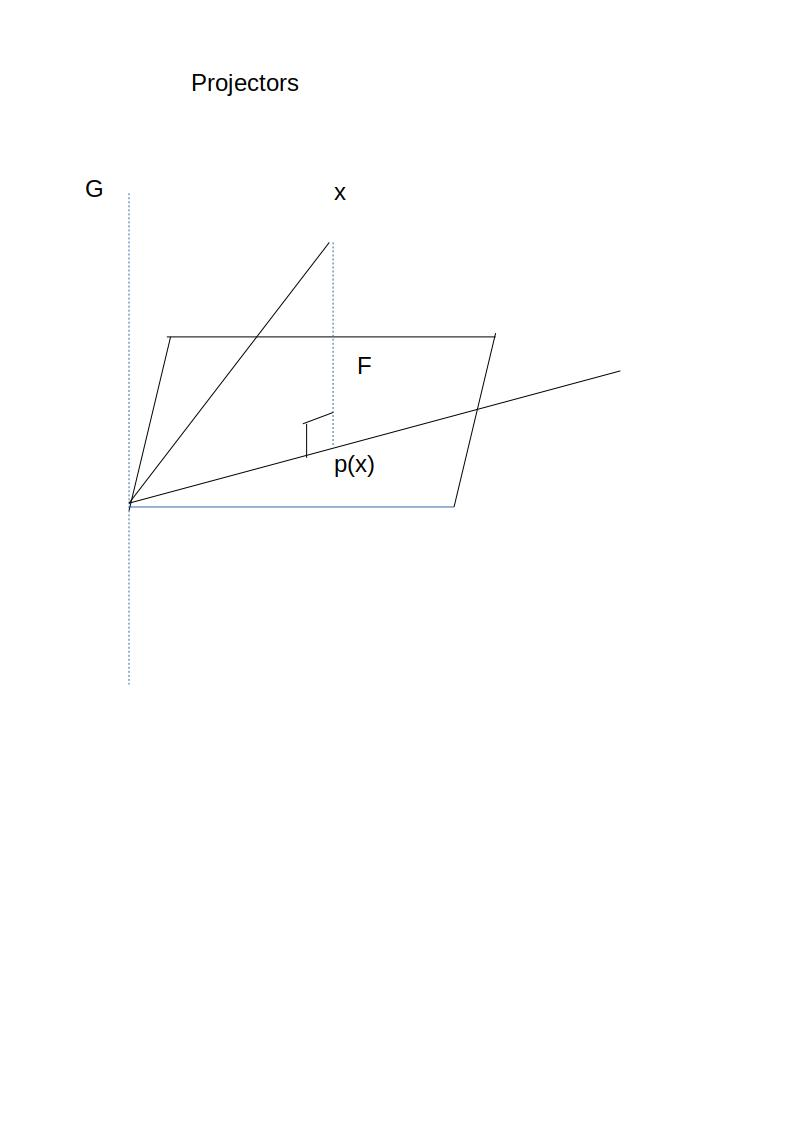
\includegraphics{Projectors.jpeg}
